%!TEX TS-program = xelatex 
%!TEX encoding = UTF-8 Unicode

% Modify the following line to match your school
% Available options include `Harvard`, `Princeton`, and `NYU`.
\documentclass[School=Harvard]{Dissertate}

\usepackage[utf8]{inputenc}
\usepackage{csquotes}


% \usepackage[a4paper, total={7in, 9in}]{geometry}
\usepackage{listings}
\usepackage{soul}
% \usepackage[sorting=none]{biblatex}
%     \addbibresource{references.bib}
% \usepackage{natbib} % has a nice set of citation styles and commands
%     \bibliographystyle{plainnat}
%     \renewcommand{\bibsection}{\subsubsection*{References}}

\usepackage{hyperref}
\usepackage{algorithm}
\usepackage{algpseudocode}
\usepackage{subfig}
\usepackage{xcolor}



\newcommand{\vect}[1]{\mathbf{#1}}
% \newcommand{\eq}[1]{Eq. \ref{#1}}
\newcommand{\px}[1]{\cfrac{\partial #1}{\partial x}}
\newcommand{\py}[1]{\cfrac{\partial #1}{\partial y}}
\newcommand{\dx}[1]{\cfrac{\mathrm{d} #1}{\mathrm{d} x}}
\renewcommand{\d}{\mathrm{d}}
\newcommand{\dy}[1]{\cfrac{\mathrm{d} #1}{\mathrm{d} y}}
\newcommand{\dt}[1]{\cfrac{\mathrm{d} #1}{\mathrm{d} t}}
\newcommand{\ds}[1]{\cfrac{\mathrm{d} #1}{\mathrm{d} s}}
\newcommand{\dnt}[2]{\cfrac{\mathrm{d}^{#1} #2}{\mathrm{d} t^{#1}}}
% \newcommand{\Err}{\mathcal{E}}
\newcommand{\Err}{\eta}
\newcommand{\Bound}{\mathcal{B}}
\newcommand{\Loss}{\mathrm{Loss}}
\newcommand{\Net}{\mathrm{Net}}
\renewcommand{\L}{\mathcal{L}}
\newcommand{\I}{\mathcal{I}}
\newcommand{\Int}[1]{e^{#1 t} \int_{0}^{t} e^{- #1 \tau}\mathrm{d}\tau}
\newcommand{\Intt}{\int_{0}^{t}\mathrm{d}\tau}
\renewcommand{\Re}[1]{\mathcal{R}e\left(#1\right)}
\newcommand{\abs}{|\cdot|}
\newcommand{\E}[1]{\mathbb{E}\left[#1\right]}
\renewcommand{\P}[1]{\mathrm{Pr}\left(#1\right)}
\DeclareMathOperator*{\argmin}{arg\,min}


\begin{document}

% the front matter
% Some details about the dissertation.
\title{Residual-Based Error Bound for Physics-Informed Neural Networks}
\author{Shuheng Liu}
\advisor{Pavlos Protopapas}

% ... about the degree.
\degree{Master of Engineering}
\field{Computational Science and Engineering}
\degreeyear{2023}
\degreemonth{May}
\department{Institute for Applied Computational Science}

% ... about the candidate's previous degrees.
\pdOneName{B.S.}
\pdOneSchool{Boston University}
\pdOneYear{2018}

\pdTwoName{M.A.}
\pdTwoSchool{Monster's Univeristy}
\pdTwoYear{2021}
\maketitle
\copyrightpage
\abstractpage
\tableofcontents
%\authorlist
\listoffigures
\dedicationpage
\acknowledgments

\doublespacing

% include each chapter...
\setcounter{chapter}{-1}  % start chapter numbering at 0
\chapter{Introduction}
\label{chapter:introduction}

Differential equations (DEs) are a useful mathematical tool for describing various phenomena in natural sciences, engineering, and humanity studies. 
As universal approximators, neural networks are powerful in approximating unknown functions. 
With back-propagation and modern computing devices, neural networks are convenient to differentiate, making them an ideal choice for solving differential equations.

However, a major criticism of neural network solutions to DEs is the lack of error bound. 
Traditional numerical methods, such as the finite difference method (FDM) and the finite element method (FEM), compute numerical solutions with known error bounds.
Unlike traditional methods, the error bounds of neural network solutions are not well-studied.
Therefore, solving DEs with neural networks requires ad hoc customization and empirical hyperparameter finetuning.
If the error of \textit{any} given network can be bounded, we can train neural networks until the error falls below a specified tolerance threshold.

Our contribution is that we propose rigorous error-bounding algorithms for any neural network solution to certain classes of equations, including linear ODEs, certain nonlinear ODEs, and first-order linear PDEs.
These algorithms can also be extended to bound the error of other classes of equations as well.
The proposed algorithms only use residual information and equation structure as inputs and do not rely on assumptions of finetuning.

The structure of this paper is as follows.
\begin{itemize}
    \item Chapter \ref{chapter:symbols-and-notations} introduces the symbols and notations adopted in this paper.
    \item Chapter \ref{chapter:literature-review} reviews the literature on emerging areas of research that are relevant to solving differential equations with neural networks.
    \item Chapter \ref{chapter:existing-work} explains the existing effort to bounding the error of neural network solutions.
    \item Chapters \ref{chapter:error-bound-for-linear-odes} and \ref{chapter:error-bound-for-nonlinear-ode} propose four algorithms for the error bound of linear and nonlinear ODEs.
    \item Chapter \ref{chapter:error-bound-for-pdes} proposes two algorithms to bound the error of first-order linear PDEs under appropriate constraint.
    \item Chapter \ref{chapter:error-bound-for-linear-sdes} proposes an algorithm to almost surely bound the error of certain linear SDEs with Gaussian noises.
    \item Chapter \ref{chapter:experiments} uses the method of manufactured solution to verify the validity of each error-bounding algorithm and provides visualization of the tightness of the bounds.
\end{itemize}
% \begin{savequote}[75mm]
% Nulla facilisi. In vel sem. Morbi id urna in diam dignissim feugiat. Proin molestie tortor eu velit. Aliquam erat volutpat. Nullam ultrices, diam tempus vulputate egestas, eros pede varius leo.
% \qauthor{Quoteauthor Lastname}
% \end{savequote}

\chapter{Symbols and Notations} \label{chapter:symbols-and-notations}
    Differential equations in this paper are posed w.r.t. unknown function $v$,
    {
        \small
        \begin{equation}
            \mathcal{D} v = f,
        \end{equation}
    }
    where $\mathcal{D}$ is a possibly nonlinear differential operator and $f$ is some forcing function.
    Unlike the exact solution $v(\cdot)$, a neural network solution $u(\cdot)$ does not strictly satisfy the equation.
    Instead, it incurs an additional residual term, $r$, which the network aims to minimize, to the equation, 
    {
        \small
        \begin{equation}
            \mathcal{D} u = f + r.
        \end{equation}
    }
    The input to $v$, $u$, $f$, and $r$ is time $t$ for ODEs and spatial coordinates $(x, y)$ for PDEs.
    We limit our reasoning to 2-dimensional PDEs in this work.
    In cases with multiple unknown functions, we use vector notations $\vect{v}$, $\vect{u}$, and $\vect{r}$ instead of the scalar notations $v$, $u$, and $r$.

\section{Loss Function}
    The loss function of the network solution is defined as the $L^2$ norm of residual $r$ over the domain of interest,
    {
        \small
        \begin{align}
            \Loss{}(u) := \frac{1}{|I|} \int_{I} \|r\|^2 \mathrm{d}I = \frac{1}{|I|} \int_{I} \|\mathcal{D} u - f\|^2 \mathrm{d}I,
        \end{align}
    }
    where a spatial domain $\Omega$ is substituted for the temporal domain $I$ in the case of a PDE.

\section{Initial and Boundary Conditions}\label{section:initial-and-boundary-conditions}
    For a neural network to satisfy initial or boundary conditions exactly, we apply a technique called \textit{parametrization}. 
    As an intuitive example, the parametrization $u(t) = (1 - e^{-t}) \Net(t) + v(0)$ guarantees that $u(t)$ satisfies the initial condition $u(0)=v(0)$ regardless of the network $\Net(\cdot)$.
    This does not affect the capability of $\Net(\cdot)$ to learn any solution.

    The parametrization is more complicated for higher-order ODEs and most PDEs and has been extensively studied by \citeauthor{lagaris1998artificial}\cite{lagaris1998artificial}, \citeauthor{lagaris2000neural}\cite{lagaris2000neural}, \citeauthor{mcfall2009artificial}\cite{mcfall2009artificial}, \citeauthor{lagari2020systematic}\cite{lagari2020systematic}, and \citeauthor{sukumar2021exact}\cite{sukumar2021exact}.
    In this work, we assume all initial and boundary conditions are exactly satisfied.

\section{Error and Error Bound}
    The error of a network solution $u$ is defined as 
    {
        \begin{equation}
            \Err = u - v.
        \end{equation}

    }
    We are interested in \textit{bounding} the error with a scalar function $\Bound$ such that 
    {
        \begin{equation}
            \|\Err(t)\| \leq \Bound(t) \quad \text{or} \quad \|\Err(x, y)\| \leq \Bound(x, y)
        \end{equation}
    }
    where $\|\Err\| = \|u - v\|$ is the \textit{absolute error}.
    If $\Bound$ takes on the same value $B \in \mathbb{R}^{+}$ over the domain, it can be replaced with a constant $B$.

    Notice that multiple bounds $\Bound$ exist for the same network solution $u$.
    For example, $|\Err(t)| \leq \Bound^{(1)}(t) \leq  \Bound^{(2)}(t) \leq \dots \leq B$ are bounds in decreasing order of tightness. Tighter bounds incur a higher computational cost, and looser bounds (such as constant $B$) are faster to compute.
% \begin{savequote}[75mm]
% Nulla facilisi. In vel sem. Morbi id urna in diam dignissim feugiat. Proin molestie tortor eu velit. Aliquam erat volutpat. Nullam ultrices, diam tempus vulputate egestas, eros pede varius leo.
% \qauthor{Quoteauthor Lastname}
% \end{savequote}

\chapter{Error Bound for Linear ODE}  \label{chapter:error-bound-for-linear-odes}
    This chapter and the next chapter consider linear and nonlinear ODEs over the temporal domain $I=[0, T]$. 
    Initial conditions are imposed on $\cfrac{\mathrm{d}^k}{\mathrm{d}t^k}v(t=0)$ for $k = 0, \dots, (n - 1)$, where $n$ is the highest order of derivative terms in ODE.

    Consider the linear ODE $\L v(t) = f(t)$, where $\L$ is a linear differential operator. 
    Its neural network solution $u$ satisfies $\L u(t) = f(t) + r(t)$. 
    Since error $\Err := u - v$, there is
    {   
        \begin{equation} \label{eq:linear-error-master}
            \L \Err(t) = r(t).
        \end{equation}
    }
    With the assumption in Section \ref{section:initial-and-boundary-conditions} that $u$ satisfies the initial conditions at $t=0$, there is
    {
        \begin{equation} \label{eq:linear-error-initial-condition}
            \Err(0) = 0, \quad \dt{}{}\Err(0) = 0, \quad \dnt{2}{}\Err(0) = 0, \quad \dots 
        \end{equation}
    }
    With initial conditions \eqref{eq:linear-error-initial-condition} known, a unique inverse transform $\L^{-1}$to $\L$ exists. 
    Applying $\L^{-1}$ to Eq. \eqref{eq:linear-error-master}, there is 
    {
        \begin{equation}\label{eq:linear-error-inverse-master}
            \Err(t) = \L^{-1} r(t).
        \end{equation}
    }
    Hence, bounding the absolute error $\left|\Err\right|$ is equivalent to bounding $\left|\L^{-1} r\right|$. 
    Notice that only a) the equation structure $\L$ and b) the residual information $r$ are relevant to estimating the error bound. 
    All other factors, including parameters of the neural network $u$, forcing function $f$, and initial conditions, do not affect the error bound at all.

\section{Single Linear ODE with Constant Coefficients}\label{section:single-linear-ode-with-constant-coefficients}
    Consider the case where $\displaystyle \L = \dnt{n}{} + \sum_{j=0}^{n - 1} a_j \dnt{j}{}$ consists of only constant coefficients $a_0, a_1, \dots, \in \mathbb{R}$.
    The characteristic polynomial of $\L$ (defined below) can be factorized into
    {
        \begin{equation} \label{eq:single-linear-ode-characteristic-polynomial-factorization}
            \lambda^n + a_{n-1}\lambda^{n-1} + \dots + a_0 = \prod_{j=1}^{n}(\lambda - \lambda_j),
        \end{equation}
    }
    where $\lambda_1, \dots, \lambda_n \in \mathbb{C}$ are the characteristic roots. 

    It is shown in Appendix \ref{appendix:proof-of-tight-and-loose-bounds} that, for a semi-stable system ($\Re{\lambda_j} \leq 0$ for all $\lambda_j$), an error bound can be formulated as
    \begin{equation} \label{eq:linear-ode-const-loose-bound}
        \left|\Err(t)\right| \leq \Bound_{loose}(t) := C_{\lambda_{1:n}}\, R_{\max}\, t^{Z},
    \end{equation}
    where $0\leq Z \leq n$ is the number of $\lambda_j$ whose real part is $0$, $\displaystyle C_{\lambda_{1:n}} := \frac{1}{Z!}\prod_{j=1; \lambda_j\neq 0}^{n} \frac{1}{\Re{-\lambda_j}}$ is a constant coefficient, and $\displaystyle R_{\max}:=\max_{t\in I} |r(t)|$ is the maximum absolute residual over domain. 
    Knowing bound \eqref{eq:linear-ode-const-loose-bound} is sufficient to qualitatively estimate the error for applications where only the order of error is concerned. See Alg. \ref{alg:single-linear-ode-constant-coeff-loose} for reference.

    \begin{algorithm}
        \caption{Loose Error Bound Estimation for Linear ODE with Constant Coefficients\quad (Requires Semi-Stability)}\label{alg:single-linear-ode-constant-coeff-loose}
        \textbf{Input:} Coefficients $\left\{a_j\right\}_{j=0}^{n-1}$ for operator $\L$, residual information $r(\cdot)$, domain of interest $I = [0, T]$, and a sequence of time points $\left\{t_\ell\right\}_{\ell=1}^{L}$ where error bound is to be evaluated\\
        \textbf{Output:} Error bound at given time points $\left\{\Bound(t_\ell)\right\}_{\ell=1}^{L}$
        \begin{algorithmic}
            \Require $\L$ is semi-stable, and $t_\ell \in I$ for all $\ell$
            \Ensure $\left|\Err(t_\ell)\right| \leq \Bound(t_\ell)$ for all $\ell$
            \State $\{\lambda_j\}_{j=1}^{n} \gets$ numerical roots of $\lambda^n+a_{n-1}\lambda^{n-1}+\dots=0$ 
            \State \textbf{assert} $\lambda_j \leq 0$ for $1 \leq j \leq n$ 
            \State $Z, C \gets 0, 1$
            \For{$j\gets 1\dots n$}
                \If{$\Re{\lambda_j} = 0$}
                    \State $Z \gets Z + 1$
                \Else
                    \State $C \gets C / \Re{-\lambda_j}$
                \EndIf
            \EndFor
            \State $R_{\max} \gets \max_{\tau \in I} |r(\tau)|$ \Comment{Use linspace with mini-steps}
            \State $\left\{\Bound(t_\ell)\right\}_{\ell=1}^{L} \gets \left\{\frac{C}{Z!}R_{\max}\, t_\ell^{Z}\right\}_{\ell=1}^{L}$
            \State \textbf{return} $\left\{\Bound(t_\ell)\right\}_{\ell=1}^{L}$
        \end{algorithmic}
        \vspace{0.5em} 
        \textbf{Note}: Polynomial roots are solvable with \citeauthor{jenkins1970three} \cite{jenkins1970three}.
    \end{algorithm}

    An issue with Eq. \eqref{eq:linear-ode-const-loose-bound} and Alg. \ref{alg:single-linear-ode-constant-coeff-loose} is that they assume $\Re{\lambda_j} \leq 0$ for all characteristic roots $\lambda_j$. 
    To address this issue, we propose an alternative error-bounding Alg. \ref{alg:single-linear-ode-constant-coeff-tight}, which requires more computation but does not require the system to be semi-stable and provides a tighter bound.

    Notice that the bounds of $\Err$ in Eq. \eqref{eq:linear-error-inverse-master} can be estimated if the inverse operator $\L^{-1}$ is known. 
    Let Eq. \eqref{eq:single-linear-ode-characteristic-polynomial-factorization} be the factorization of characteristic polynomial of $\L$.
    Define operator $\I_{\lambda}$ as
    \begin{equation} \label{eq:integral-operator-definition}
        \I_\lambda \psi(t) := e^{{\lambda} t} \int_{0}^{t} e^{-{\lambda} \tau} \psi(\tau) \mathrm{d}\tau, \quad \forall \psi : I \to \mathbb{C}.
    \end{equation}
    It is shown in Appendix \ref{appendix:inverse-operator} that,
    \begin{equation} \label{eq:single-linear-ode-inverse-operator-factorization}
        \L^{-1} = \I_{\lambda_{n}} \circ \I_{\lambda_{n-1}} \circ \dots \circ \I_{\lambda_1}
    \end{equation} 
    and that 
    \begin{equation} \label{eq:inverse-operator-inequality}
        \left|\I_{\lambda} \psi\right| \ \leq \I_{\Re{\lambda}} |\psi| \quad \text{for all }\lambda \in \mathbb{C}, \text{ and } \psi : I \to \mathbb{C}.
    \end{equation} 
    Hence, another error bound can be formulated as
    \begin{equation} \label{eq:single-linear-ode-inverse-operator-inequality}
        \Bound_{tight}(t) := \left(\I_{\Re{\lambda_{n}}} \circ \dots \circ \I_{\Re{\lambda_1}}\right) |r(t)|.
    \end{equation}
    It is proven in Appendix \ref{appendix:proof-of-tight-and-loose-bounds} that $\Bound_{tight}$ is tighter than $\Bound_{loose}$ when $\Bound_{loose}$ is applicable,
    \begin{equation} \label{eq:single-linear-ode-tight-and-loose}
        \left|\Err(t)\right| \leq \Bound_{tight}(t) \leq \Bound_{loose}(t) \quad \forall t \in I.
    \end{equation}
    Based on Eq. \eqref{eq:single-linear-ode-inverse-operator-inequality}, we propose Alg. \ref{alg:single-linear-ode-constant-coeff-tight}, which computes $\Bound_{tight}$ by repeatedly evaluating integrals in \eqref{eq:integral-operator-definition} using the cumulative trapezoidal rule.

    \begin{algorithm}
        \caption{Tighter Error Bound Estimation for Linear ODE with Constant Coefficients\quad  (Stable and Unstable)}\label{alg:single-linear-ode-constant-coeff-tight}
        \textbf{Input \& Output:} Same as Alg. \ref{alg:single-linear-ode-constant-coeff-loose}
        \begin{algorithmic}
            \Require Same as Alg. \ref{alg:single-linear-ode-constant-coeff-loose}, except $\L$ can be unstable
            \Ensure Same as Alg. \ref{alg:single-linear-ode-constant-coeff-loose}
            \State $\{\lambda_j\}_{j=1}^{n} \gets$ numerical roots of $\lambda^n+a_{n-1}\lambda^{n-1}+\dots=0$
            \State $\left\{t_k\right\}_{k=0}^{K} \gets$ linspace($0$, $T$, \normalfont{sufficient steps})
            \State $\left\{\Bound(t_k)\right\}_{k=0}^{K} \gets \left\{|r(t_k)|\right\}_{k=0}^{K}$
            \For{$j \gets 1 \dots n$}
                \State integral$_{k=0}^{K} \gets$ CumTrapz($\left\{e^{-\lambda_j t_{k}} \Bound(t_k)\right\}_{k=0}^{K}$, $\left\{t_k\right\}_{k=0}^{K}$) 
                \State $\left\{\Bound(t_k)\right\}_{k=0}^{K} \gets \left\{e^{\lambda_j t_{k}}\cdot \text{integral}_k \right\}_{k=0}^{K}$ 
            \EndFor
            \State $\left\{\Bound(t_\ell)\right\}_{\ell=1}^{L} \gets $ Interpolate($\left\{\Bound(t_k)\right\}_{k=0}^{K}$, $\left\{t_k\right\}_{k=0}^{K}$, $\left\{t_\ell\right\}_{\ell=0}^{L}$) 
            \State \textbf{return} $\left\{\Bound(t_\ell)\right\}_{\ell=1}^{L}$ 
        \end{algorithmic}

        \vspace{0.5em} 
        \textbf{Note}: CumTrapz($\{y_k\}_{k=1}^K$, $\{x_k\}_{k=1}^K$) computes cumulative integral $\int_{0}^x y(x)\mathrm{d}x$ at discrete points $\{x_k\}_{k=1}^K$ using trapezoidal rule.\\
        \textbf{Note}: Interpolate($\{y_k\}_{k=1}^K$, $\{x_k\}_{k=1}^K$, $\{x_\ell\}_{\ell=1}^L$) computes interpolant to a function with given discrete data points $\{(x_k, y_k)\}_{k=1}^K$ evaluated at $\{x_\ell\}_{\ell=1}^L$.
    \end{algorithm}

\section{Single Linear ODE of the General Form}
   In general, the coefficients for $\L$ can be functions of $t$. Namely, $\displaystyle \L = \dnt{n}{} + \sum_{j=0}^{n-1}a_j(t)\dnt{j-1}{}$.
   Similar to Eq. \eqref{eq:single-linear-ode-characteristic-polynomial-factorization}, $\L$ have characteristic roots $\{\lambda_{j}(t)\}_{j=1}^{n}$ as functions of $t$,
    {
        \begin{equation*} \label{eq:functional-factorization}
            \lambda^n + a_{n-1}(t)\lambda^{n-1} + \dots + a_0(t) = \prod_{j=1}^{n}(\lambda - \lambda_j(t)).
        \end{equation*}
    }
    We can replace constant $\lambda_j$ with functions $\lambda_j(t)$ in Eq. \eqref{eq:integral-operator-definition} and compute bound $\Bound_{tight}$ as in Eq. \eqref{eq:single-linear-ode-inverse-operator-inequality}.
    However, the factorization in Eq. \eqref{eq:functional-factorization} is hard to implement in practice except for the first-order case  where $\L v = \frac{\mathrm{d}v}{\mathrm{d}t} + a_0(t)v$. 
    Cases of second order and higher are out of the scope of this paper.

\section{System of Linear ODEs with Constant Coefficients} \label{section:system-of-linear-odes-with-constant-coefficients}
    Consider a system of linear ODEs with constant coefficients 
    {
        \begin{equation}\label{eq:linear-system-master}
            \frac{\mathrm{d}}{\mathrm{d}t}\vect{v} + A\vect{v} = \vect{f}(t)
        \end{equation}
    }
    where $\vect{v}$ and $\vect{f}$ are $\mathbb{R}^n$ vectors and $A$ is a $n\times n$ matrix. Denote the Jordan canonical form of $A$ as,
    {
        \begingroup 
        \setlength\arraycolsep{1pt}
        \begin{equation}\label{eq:jordan-definition}
            J = P^{-1}AP= \begin{pmatrix}
                J_1 \quad & & \\
                & \ddots & \\
                & & \quad J_K
            \end{pmatrix}
            {\quad \text{ where }\quad }
            J_k = \begin{pmatrix}
                \lambda_k & 1\\[-0.75em]
                & \lambda_k & \ddots\\[-0.75em]
                & & \ddots & 1\\[-0.25em]
                & & & \lambda_k
            \end{pmatrix}.
        \end{equation}
        \endgroup
    }
    Let $n_k$ be the size of Jordan block $J_k$, we construct an operator matrix $\pmb{\I} = \text{diag}(\vect{I}_1, \vect{I}_2, \dots)$, where 
    {
        \begingroup 
        \setlength\arraycolsep{1pt}
        \begin{equation}\label{eq:operator-block}
            \vect{I}_k = \begin{pmatrix}
                \I_{-\Re{\lambda_k}} & \I_{-\Re{\lambda_k}}^2 & \dots &\I_{-\Re{\lambda_k}}^{n_k} \\[1ex]
                0 & \I_{-\Re{\lambda_k}} & \dots &\I_{-\Re{\lambda_k}}^{n_k-1} \\[-1ex]
                \vdots & \vdots & \ddots & \vdots \\
                0 & 0 & \dots & \I_{-\Re{\lambda_k}}
            \end{pmatrix}.
        \end{equation}
        \endgroup
    }
    An \textit{elementwise bound} (vector) $\pmb{\Bound}(t)$ can be formulated as 
    {
        \begin{equation}\label{eq:system-component-bound}
            \pmb{\Err}^{\abs}(t) \preceq \pmb{\Bound}(t) := P^{\abs} \pmb{\I}\left[(P^{-1})^{\abs} \ \vect{r}^{\abs}\right](t),
        \end{equation}
    }
    where superscript $\abs$ denotes taking elementwise absolute value and symbol $\preceq$ denotes elementwise inequality. In the meantime, a \textit{norm bound} (scalar) $\Bound(t)$ also exists
    {
        \begin{equation}\label{eq:system-norm-bound}
            \left\|\pmb{\Err}(t)\right\| \leq \Bound(t) := \mathrm{cond}(P)\left\|\pmb{\I}\big[\|\vect{r}\|\vect{1}\big](t)\right\|
        \end{equation}
    }
    where $\mathrm{cond}(P)$ is the conditional number of $P$ w.r.t. induced matrix norm, and $\vect{1}$ is an $n\times 1$ column vector of $1$s. 
    Proof of Eq. \eqref{eq:system-component-bound} and Eq. \eqref{eq:system-norm-bound} can be found in Appendix \ref{appendix:proof-of-bounds-for-ode-systems}.
    See Alg. \ref{alg:system-bound} for implementation.

    \begin{algorithm}
        \caption{ODE System Bound (norm and elementwise)}\label{alg:system-bound}
        \textbf{Input:} Coefficient matrix $A \in \mathbb{R}^{n\times n}$, residual vector $\vect{r}(t)$, and a sequence of points $\left\{t_\ell\right\}_{\ell=1}^{L}$ where error is to be bounded\\
        \textbf{Output:} Norm bound (scalar) $\left\{\Bound(t_\ell)\right\}_{\ell=1}^{L}$ and componentwise bound (vector) $\left\{\pmb{\Bound}(t_\ell)\right\}_{\ell=1}^{L}$ at given time points
        \begin{algorithmic}
            \Ensure $\|\Err(t_\ell)\| \leq \Bound(t_\ell)$ and $\Err(t_\ell) \preceq \pmb{\Bound}(t_\ell)$ for all $\ell$

            \State $J, P \gets $ Jordan canonicalization of $A = PJP^{-1}$
            % \State $\vect{I} \gets$ construct matrix operator $\vect{I}$ using Eq. \eqref{eq:operator-block}
            \For{each Jordan block $J_k$ of shape $n_k \times n_k$}
                \State $\vect{I}_k \gets$ construct operator block using Eq. \eqref{eq:operator-block} 
            \EndFor
            \State $\pmb{\I} \gets$ diag($\vect{I}_1$, $\vect{I}_2$,  \dots)
            \State $\left\{\pmb{\Bound}(t_\ell)\right\}_{\ell=1}^{L} \gets \{P^{\abs} \pmb{\I}\big[(P^{-1})^{\abs} \vect{r}^{\abs}\big](t_\ell)\}_{\ell=1}^{L}$
            \State $\left\{\Bound(t_\ell)\right\}_{\ell=1}^{L} \gets \{\mathrm{cond}(P)\left\|\pmb{\I}\big[\|\vect{r}\|\vect{1}\big](t_\ell)\right\|\}_{\ell=1}^{L}$
            \State \textbf{return} $\left\{\Bound(t_\ell)\right\}_{\ell=1}^{L}$, $\left\{\pmb{\Bound}(t_\ell)\right\}_{\ell=1}^{L}$
        \end{algorithmic}
    \end{algorithm}


\chapter{Error Bound for Nonlinear ODE}\label{chapter:error-bound-for-nonlinear-ode}
    Nonlinear ODEs can be hard to solve and bound in general.
    In this work, we only deal with nonlinear ODEs with a single nonlinear term of the form $\varepsilon v^k(t)$, where $\varepsilon \in \mathbb{R}$ controls the strength of the nonlinearity.
    Ideally, a nonlinear term with $|\varepsilon| \ll 1$ is easier to solve and bound, which is assumption of our derivations. 
    With the perturbation technique, we obtain a family of solutions $v(t;\varepsilon)$ parameterized by $\varepsilon$ at the cost of solving a (countable) collection of equations. 
    As explained below in section \ref{section:perturbation-theory}, we train finitely many networks, each approximately solving an equation in the collection.

\section{Perturbation Theory} \label{section:perturbation-theory}
    Consider the nonlinear ODE with nonlinear term $\varepsilon v^k(t)$,
    {
        \begin{equation} \label{eq:nonlinear-ode-master}
            \L v(t) + \varepsilon v^k(t) = f(t),
        \end{equation}
    }
    where $\L$ is a linear differential operator discussed in \ref{section:error-bound-for-linear-odes} and initial conditions are specified for the system at time $t=0$. 
    Notice that each $\varepsilon \in \mathbb{R}$ corresponds to a solution $v(t; \varepsilon)$. 
    We expand the solution $v(t; \varepsilon)$ in terms of $\varepsilon$
    {   
        \begin{equation} \label{eq:nonlinear-solution-expansion}
            v(t; \varepsilon) = \sum_{j=0}^{\infty} \varepsilon^j v_j(t) = v_0(t) + \varepsilon v_1(t) + \dots
        \end{equation}
    }
    Only $v_0(t)$ is subject to the original initial conditions at $t=0$, while other components, $v_1$, $v_2$, \dots, have initial conditions of $0$ at $t=0$.
    Substituting Eq. \eqref{eq:nonlinear-solution-expansion} into Eq. \eqref{eq:nonlinear-ode-master}, there is
    {
        \begin{gather}
            \L \sum_{j=0}^{\infty} \varepsilon^j v_j + \varepsilon \left(\sum_{j=0}^{\infty} \varepsilon^j v_j\right)^k = f \\
            % \sum_{j=0}^{\infty} \varepsilon^j \L v_j + \varepsilon \left(\sum_{j=0}^{\infty} \varepsilon^j v_j\right)^k = f \\
            \sum_{j=0}^{\infty} \varepsilon^j \L v_j + \sum_{j=0}^{\infty} \varepsilon^{j+1} \sum_{\substack{j_1+\dots+j_k = j\\j_1, \dots, j_k \geq 0}}v_{j_1}\dots v_{j_k} = f \\[-0.5em]
            \L v_0 + \sum_{j=1}^{\infty} \varepsilon^j \Bigg(\L v_j + \sum_{\substack{j_1+\dots+j_k = j - 1\\j_1, \dots, j_k \geq 0}}v_{j_1}\dots v_{j_k}\Bigg)= f \label{eq:nonlinear-equation-expansion} 
        \end{gather}
    }
    In order for Eq. \eqref{eq:nonlinear-equation-expansion} to hold true for all $\varepsilon$, the coefficients for each $\varepsilon^j$ must match on both sides of Eq. \eqref{eq:nonlinear-equation-expansion}. Hence,
    {
        \begin{alignat}{6}
            &\L v_0 &&= f \label{eq:expansion-epsilon-0}\\
            &\L v_1 + v_0^k &&= 0 \label{eq:expansion-epsilon-1}\\
            &\L v_2 + k v_0^{k-1}v_1 &&= 0 \label{eq:expansion-epsilon-2} \\
            &\L v_3 + \frac{k(k-1)}{2} v_0^{k-2}v_1^2 + k v_0^{k-1}v_2 &&= 0 \label{eq:expansion-epsilon-3} \\[-1em]
            &\vdots &&\phantom{=}\,\,\,\,\vdots\nonumber
        \end{alignat}
    }

    For $\varepsilon = 0$, Eq. \eqref{eq:nonlinear-solution-expansion} is reduced to $v_0(t)$, which solves the linear problem $\L v=f$. 

    \begingroup
        \setlength{\itemsep}{0pt}
        \setlength{\parskip}{0pt}
        The above system can be solved in a \textit{sequential} manner, either analytically or using neural networks,
        \begin{enumerate}
            \item Eq. \eqref{eq:expansion-epsilon-0} is linear in $v_0$ and can be solved first. 
            \item With $v_0$ known, Eq. \eqref{eq:expansion-epsilon-1} is linear in $v_1$ and can be solved for $v_1$. 
            \item Similarly, with $v_0$ and $v_1$ known, Eq. \eqref{eq:expansion-epsilon-2} is linear in $v_2$ and can be solved for $v_2$.
            \item The process can be repeated for Eq. \eqref{eq:expansion-epsilon-3} and beyond. Only a linear ODE is solved each time.
        \end{enumerate}
        To solve the system with PINNs, we approximate exact solutions $\left\{v_j(t)\right\}_{j=1}^{\infty}$ with neural network solutions $\left\{u_j(t)\right\}_{j=0}^{J}$ trained sequentially on Eq. \eqref{eq:expansion-epsilon-0}, Eq. \eqref{eq:expansion-epsilon-1}, and beyond. 
        In practice, we only consider components up to order $J$ to avoid the infinity in expansion \eqref{eq:nonlinear-solution-expansion}. 
        Ideally, $J$ should be large enough so that higher order residuals in expansion \eqref{eq:nonlinear-solution-expansion} can be neglected.
    \endgroup

    After obtaining $\left\{u_j(t)\right\}_{j=0}^{J}$, we can reconstruct the solution $u(t;\varepsilon) = \sum_{j=0}^{J} \varepsilon^j u_j(t)$ to the original nonlinear equation \eqref{eq:nonlinear-ode-master} for varying $\varepsilon$.
    See Alg. \ref{alg:nonlinear-iterative} for details.

\section{Expansion of Bounds}
    The absolute error $|\Err(t;\varepsilon)| = |u(t;\varepsilon) - v(t;\varepsilon)|$is given by 
    {
        \begin{align}
            |\Err(t; \varepsilon)| %&= \big|u(t; \varepsilon) - v(t; \varepsilon)\big| \nonumber \\[-0.25em]
            &= \left|\sum_{j=0}^{J} \varepsilon^{j} \Big(u_j(t) - v_j(t)\Big) - \sum_{j=J+1}^{\infty} \varepsilon^j v_j(t)\right| \nonumber \\[-0.5em]
            &\leq \sum_{j=0}^{J} \Big|\Err_{j}(t)\Big||\varepsilon|^j + \left|\sum_{j=J+1}^{\infty}\varepsilon^j v_j(t)\right| 
        \end{align}
    }
    where $\Err_{j}(t) := u_j(t) - v_j(t)$ is the \textit{component error} between $u_j(t)$ and $v_j(t)$.
    Let $\Bound_{j}$ denote the \textit{bound component} such that $|\Err_{j}(t)| \leq \Bound_j(t)$.
    Assuming $J$ is large and higher order terms $\left|\sum_{j=J+1}^{\infty}\varepsilon^j v_j(t)\right|$ are negligible, there is 
    {
        \begin{equation} \label{eq:nonlinear-bound-components}
            \Big|\Err(t; \varepsilon)\Big| \leq \Bound(t; \varepsilon) := \sum_{j=0}^{J} \Bound_j(t)\,|\varepsilon|^j 
        \end{equation}
    }
    where each bound component $\Bound_j$ can be evaluated using the techinque in Section \ref{section:error-bound-for-linear-odes}. 
    See Alg. \ref{alg:nonlinear-iterative} for details.

    \makeatletter
    \setlength{\@fptop}{0pt}
    \begin{algorithm}
        \caption{Iterative Method for Solution and Error Bound of Nonlinear ODE \eqref{eq:nonlinear-ode-master}} \label{alg:nonlinear-iterative}
        \textbf{Input:} Linear operator $\L$, nonlinear degree $k$, domain $I=[0, T]$, highest order $J$ for expansion, and a sequence $\left\{(t_\ell, \varepsilon_\ell)\right\}_{\ell=1}^{L}$ where solution $u(t; \varepsilon)$ and error bound $\Bound(t; \varepsilon)$ are to be evaluated \\
        \textbf{Output:} Solution $\left\{u(t_\ell; \varepsilon_\ell)\right\}_{\ell=1}^{L}$ and error bound $\left\{\Bound(t_\ell; \varepsilon_\ell)\right\}_{\ell=1}^{L}$ 
        \begin{algorithmic}
            \Require $t_\ell \in I$, and $|\varepsilon_\ell|$ to be small (ideally $|\varepsilon_\ell| \ll 1$)
            \Ensure $\Err(t_\ell; \varepsilon_\ell) \leq \Bound(t_\ell; \varepsilon_\ell)$ 

            \State $u_0, r_0, \gets$ network solution, residual of $\L u_0 = f$
            \State $\left\{\Bound_{0}(t_\ell)\right\}_{\ell=1}^L \gets$ bound of $\left|\L^{-1}r_0\right|$ at $\left\{t_\ell\right\}_{\ell=1}^L$
            \For{$j \gets 1 \dots J$} 
                \State Define macro $\text{NL}_j[\phi]$ as $\sum_{\substack{j_1 + \dots + j_k = j-1\\ j_1, \dots, j_k \geq 0}} \phi_{j_1} \dots \phi_{j_k}$
                \State $u_j, r_j \gets$ network solution, residual of $\L u_j + \text{NL}_j[u] = 0$
                \State $\Bound_{\text{NL}} \gets \text{upper bound of }|\text{NL}_j[u] - \text{NL}_j[v]|$
                \State $\left\{\Bound_{j}(t_\ell)\right\}_{\ell=1}^L \gets$  bound of $|\L^{-1}r_j|$+$|\L^{-1}\Bound_{\text{NL}}|$ at $\left\{t_\ell\right\}_{\ell=1}^L$
            \EndFor
            \State $\left\{u(t_\ell; \varepsilon_\ell)\right\}_{\ell=1}^L \gets \big\{\sum_{j=0}^{J}\varepsilon_\ell^j u_j(t_\ell)\big\}_{\ell=1}^L $ 
            \State $\left\{\Bound(t_\ell; \varepsilon_\ell)\right\}_{\ell=1}^L \gets \big\{\sum_{j=0}^{J}\varepsilon_\ell^j \Bound_j(t_\ell)\big\}_{\ell=1}^L $ 
            \State \textbf{return} $\left\{u(t_\ell; \varepsilon_\ell)\right\}_{\ell=1}^L, \left\{\Bound(t_\ell; \varepsilon_\ell)\right\}_{\ell=1}^L$
        \end{algorithmic}
        \vspace{0.5em}

        \textbf{Note} 1: $\Bound_0(t)$ and $\Bound_{1:J}(t)$ can be evaluated using either Alg. \ref{alg:single-linear-ode-constant-coeff-loose} or \ref{alg:single-linear-ode-constant-coeff-tight}.\\
        \textbf{Note} 2: $\Bound_\text{NL}$ can be estimated even though exact solutions $v_{0:j-1}(t)$ are unknown. This is because $ u_i(t) - \Bound_i(t) \leq v_i(t) \leq u_i(t)+\Bound_i(t)$ for all $i$, and $u_{0:j-1}(t)$, $\Bound_{0:j-1}(t)$ are known from previous iterations.
    \end{algorithm}
    \makeatother
\chapter{Error Bound for First-Order Linear PDE} \label{chapter:error-bound-for-pdes}
    This chapter considers first-order linear PDEs defined on a 2-dimensional spatial domain $\Omega$,\footnote{Similar techniques can be used for other classes of PDEs and higher dimensions where the method of characteristics applies.} 
    % Consider the first-order linear PDE,
    { 
        \begin{equation}\label{eq:pde-master}
            a(x, y) \px{v} + b(x, y) \py{v} + c(x, y)v = f(x, y)
        \end{equation}
    }
    with Dirichlet boundary constraints defined on $\Gamma \subset \partial \Omega$,
    {
        \begin{equation}\label{eq:pde-bc-master}
            v\big|_{(x, y) \in \Gamma} = g(x, y).
        \end{equation}
    }

    We partition the domain into infinitely many characteristic curves $\mathcal{C}$, each passing through a point $(x_0, y_0) \in \Gamma$. The resulting curve is a parameterized integral curve 
    {
        \begin{equation*} 
            \mathcal{C}: \begin{cases*}
                x'(s) = a(x, y) \\
                y'(s) = b(x, y) 
            \end{cases*} 
            \quad
            \text{where}
            \,\,
            (\cdot)' = \ds{}
            \quad
            \text{and} 
            \quad
            \begin{aligned}
                x(0) &= x_0 \\
                y(0) &= y_0.
            \end{aligned}
        \end{equation*}
    }
    % Note that the system \eqref{eq:parameter-eq-differential} can be nonlinear but needs not always be solved for a loose error bound to be evaluated. 
    % Still, knowing the exact characteristic curves $\mathcal{C}$ leads to a tighter bound.
    For any $(x(s), y(s))$ on $\mathcal{C}$, functions $v, a, b, c$, and $f$ can be viewed as univariate functions of $s$. By chain rule, there is
    {
        
        \begin{equation*}
            a(x, y)\px{v} + b(x, y)\py{v} = x'(s)\px{v}  + y'(s)\py{v} = v'(s).
        \end{equation*}
    }
    Hence, Eq. \eqref{eq:pde-master} is reformulated as an ODE along curve $\mathcal{C}$,
    {
        
        \begin{equation}
            v'(s) + c(s) v(s) = f(s) \quad \text{s.t. } v(0) = g(x_0, y_0),
        \end{equation}
    }
    where $v(s)$, $c(s)$, and $f(s)$ are shorthand notations for $v(x(s),y(s))$, $c(x(s),y(s))$, and $f(x(s),y(s))$, respectively.

    In particular, if $c(x, y) \neq 0$ for all $(x, y) \in \Omega$, both sides of Eq. \eqref{eq:pde-master} can be divided by $c(x, y)$, resulting in a residual of $r(x, y)/c(x, y)$ where $r(x, y)$ is the residual of the original problem. 
    By Eq. \eqref{eq:linear-ode-const-loose-bound}, a constant error bound on $\mathcal{C}$ is $|\Err(s)| \leq \max_{s}\left|r(s)/c(s)\right|$. 
    Hence, a (loose) constant error bound $B$ (see Alg. \ref{alg:linear-first-order-pde-constant}) over the entire domain $\Omega$ is
    {
        
        \begin{equation}
            |\Err(x, y)| \leq B :=\max_{(x, y)\in \Omega}\left|\frac{r(x, y)}{c(x, y)}\right|.
        \end{equation}
    }

    \makeatletter
    \setlength{\@fptop}{0pt}
    \begin{algorithm}
        \caption{Constant Err Bound for Linear 1st-Order PDE}\label{alg:linear-first-order-pde-constant}
        \textbf{Input:} Coefficient $c(x, y)$ in Eq. \eqref{eq:pde-master}, residual information $r(x, y)$ and domain of interest $\Omega$\\
        \textbf{Output:} A constant error bound $B \in \mathbb{R}^+$
        \begin{algorithmic}
            \Require $c(x, y) \neq 0$ for all $(x, y) \in \Omega$
            \Ensure $|\Err(x, y)| \leq B$ for all $(x, y) \in \Omega$

            \State $\left\{(x_k, y_k)\right\}_{k} \gets$ sufficiently dense mesh grid over $\Omega$
            \State $\displaystyle B \gets \max_{k} \left| \frac{r(x_k, y_k)}{c(x_k, y_k)}\right|$
            \State \textbf{return} $B$
        \end{algorithmic}
    \end{algorithm}
    \makeatother

    Independent of the assumption $c(x, y)\neq 0$, in scenarios where the curve $\mathcal{C}$ passing through any $(x, y)$ can be computed, the error can be computed using Alg. \ref{alg:linear-first-order-pde-general}.

    \makeatletter
    \setlength{\@fptop}{0pt}
    \begin{algorithm}
        \caption{General Err Bound for Linear 1st-Order PDE}\label{alg:linear-first-order-pde-general}
        \textbf{Input:} Coefficients $a(x, y)$, $b(x, y)$, $c(x, y)$ in Eq. \eqref{eq:pde-master}, residual information $r(x, y)$, domain of interest $\Omega$, Dirichlet boundary $\Gamma\subset \partial \Omega$, and a sequence of points $\left\{(x_\ell, y_\ell)\right\}_{\ell=1}^{L}$ where error is to be bounded\\
        \textbf{Output:} Error bound $\left\{\Bound(x_\ell, y_\ell)\right\}_{\ell=1}^{L}$ at given points
        \begin{algorithmic}
            \Require Integral curve of the vector field $\big[a(x, y)\,\, b(x, y)\big]^T$ passing through any point $(x_\ell, y_\ell) \in \Omega$ is solvable
            \Ensure $|\Err(x_\ell, y_\ell)| \leq \Bound(x_\ell, y_\ell)$ for all $\ell$

            \State $\mathcal{C}_{\text{gen}} \gets $ general solution (integral curves) to {$\begin{cases}x'(s) = a(x, y) \\ y'(s) = b(x, y)\end{cases}$}
            \For{$\ell \gets 1 \dots L$}
                \State $\mathcal{C}:(x(s), y(s))\gets$ instance of $\mathcal{C}_{\text{gen}}$ passing through $(x_\ell, y_\ell)$
                \State $s^* \gets$ solution to $x(s) = x_\ell,\, y(s)=y_\ell$
                \State $\displaystyle \Bound(x_\ell, y_\ell) \gets e^{c(s^*)}\int_{0}^{s^*}r(x(s), y(s)) e^{-c(x(s),y(s))\,s}\mathrm{d}s$ 
            \EndFor
            \State \textbf{return} $\left\{\Bound(x_\ell, y_\ell)\right\}_{\ell=1}^{L}$
        \end{algorithmic}
    \end{algorithm}
    \makeatother
\begin{savequote}[75mm]
    The theory of probability is the only mathematical tool available to help map the unknown and the uncontrollable. It is fortunate that this tool, while tricky, is extraordinarily powerful and convenient.
\qauthor{Benoit Mandelbrot}
\end{savequote}

\chapter{Error Bound for Linear SDE}  \label{chapter:error-bound-for-linear-sdes}
    In addition to deterministic differential equations, we also consider a class of linear stochastic differential equations (SDEs) in this thesis by introducing an additional stochastic term to the forcing function. 
    For any given network, we aim to bound the error at any point with arbitrary high probability using the network's residual on the deterministic part of the equation.
\section{Formulation}
    In this chapter, we deal with linear first-order SDEs of the form
    \begin{equation}\label{eq:linear-sde}
        \d V_t = \big(\lambda V_t + f(t)\big)\d t + g(t) \d W_t \quad \text{s.t.} \quad V_0 = v_0 
    \end{equation}
    where $W_t$ is a Wiener process. 
    We assume that $f(t)$ and $g(t)$ are deterministic functions and $\lambda \in \mathbb{R}$ is a constant. 
    We denote the solution with capital $V_t$ because it is a continuous stochastic process whose realization depends on the realization of $W_t$.

    Unlike with deterministic differential equations, we do not evaluate the residual $r(t)$ of a network solution $u(t)$ on the SDE because the stochastic term $g(t) \d W(t)$ is not deterministic.
    Instead, we evaluated the residual on the following deterministic differential equation
    \begin{equation}
        \E{\d V_t} = \E{\big(\lambda V_t + f(t)\big)\d t + g(t) \d W_t}
    \end{equation}
    Assuming we can change the order of expectation and differentiation, we have
    \begin{equation}
        \d v(t) = (\lambda v(t) + f(t))\d t
    \end{equation}
    where $v(t) = \E{V(t)}$. 
    Since this is a deterministic differential equation, we can evaluate the residual of neural network $u(t)$ on this equation. 
    Namely,
    \begin{equation}\label{eq:linear-sde-network}
        \d u(t) = \big( \lambda u(t) + f(t)\big) \d t + r(t)\d t.
    \end{equation}
    We aim to formulate a bound for the absolute error $|\Eta_t| = |u(t) - V_t|$ using only $\lambda$, $f(\cdot)$, and $g(\cdot)$. 
    Since the error $\Eta_t$ is a stochastic process, we shall formulate an upper tail bound for the distribution of $\Eta_t$. 
    Namely, we aim to formulate a bound $|\Eta| \leq \Bound_\epsilon$ that holds true with arbitrarily high probability $1 - \epsilon$,
    \begin{equation}\label{eq:upper-tail-bound-goal}
        \P{\, \big|\Eta_T\big| \leq \Bound_\epsilon(t)} \geq 1 - \epsilon \quad \forall t \in I.
    \end{equation}
\section{Upper Tail Bound of Absolute Error}
    To derive a tail bound Eq. \eqref{eq:upper-tail-bound-goal}, we take the difference between Eq. \eqref{eq:linear-sde-network} and Eq. \eqref{eq:linear-sde},
    \begin{equation}
        \d \Eta_t  = \big(\lambda \Eta_t + r(t)\big)\d t - g(t) \d W_t
    \end{equation}
    It is well known the the solution of this equation is
    \begin{equation}
        \Eta_t = \I_{\lambda} r(t) - e^{\lambda t} \int_0^t e^{-\lambda \tau} g(\tau) \d W_\tau
    \end{equation}
    Since $\lambda \in \mathbb{R}$, by the triangle inequality and property \eqref{eq:inverse-operator-inequality} of operator $\I_{\lambda}$, there is
    \begin{align}\label{eq:eta-bound-unevaluated}
        \big|\Eta_t\big| &\leq \big|\I_{\lambda} r(t)\big| + \left|e^{\lambda t} \int_0^t e^{-\lambda \tau} g(\tau) \d W_\tau\right|\\
        &\leq \I_{\Re{\lambda}} |r(t)| + \left|e^{\lambda t} \int_0^t e^{-\lambda \tau} g(\tau) \d W_\tau\right|\\
        &= \I_{\lambda} |r(t)| + e^{\lambda t} \left|\int_0^t e^{-\lambda \tau} g(\tau) \d W_\tau\right|\label{eq:eta-bound-unevaluated}
    \end{align}
    where the first term $\I_{\lambda} |r|$ can be bounded using either Alg. \ref{alg:single-linear-ode-constant-coeff-loose} or Alg. \ref{alg:single-linear-ode-constant-coeff-tight}.
    For the second term, notice that for almost every realization of $\d W_t$, the integral $\displaystyle \int_0^t e^{-\lambda \tau} g(\tau) \d W_\tau$ is a Riemann-Stieltjes integral and can be evaluted by parts.
    Namely, 
    \begin{align}
        e^{\lambda t} \left|\int_0^t e^{-\lambda \tau} g(\tau) \d W_\tau\right| &= e^{\lambda t} \left|  e^{-\lambda t} g(t) W_t - 1 \cdot g(0) W_0 - \int_{0}^{t} W_\tau \d \big(e^{-\lambda\tau}g(\tau)\big)\right| \\
        &= e^{\lambda t} \left|  e^{-\lambda t} g(t) W_t - \int_{0}^{t} e^{-\lambda\tau}\big(g'(\tau) - \lambda g(\tau)\big) W_\tau \d \tau\right| \\
        &= \left|  g(t) W_t - e^{\lambda t} \int_{0}^{t} e^{-\lambda\tau}\big(g'(\tau) - \lambda g(\tau)\big) W_\tau \d \tau\right| \\
        &\leq \left| g(t)W_t \right| + \left|e^{\lambda t} \int_{0}^{t} e^{-\lambda\tau}\big(g'(\tau) - \lambda g(\tau)\big) W_\tau \d \tau\right|
    \end{align}
    Let $p(\tau) = e^{-\lambda\tau}\big(g'(\tau) - \lambda g(\tau)\big)$.
    By the Cauchy-Schwarz inequality, there is
    \begin{align}
        e^{\lambda t} \left|\int_0^t e^{-\lambda \tau} g(\tau) \d W_\tau\right| &\leq \left| g(t)W_t \right| + \left|e^{\lambda t} \int_{0}^{t} p(\tau) W_\tau \d \tau\right| \\
        &\leq \left| g(t)W_t \right| + e^{\lambda t} \sqrt{\int_{0}^{t} p^2(\tau) \d \tau} \sqrt{\int_{0}^{t} W_\tau^2 \d \tau}\label{eq:bound-of-stochastic-part-unsolved}
    \end{align}
    Since $W_t$ is a Wiener process, there is $W_t \sim \mathcal{N}(0, t)$.
    It is well known that the tail bound of the normal distribution $\mathcal{N}(0, t)$ is given by
    \begin{equation}\label{eq:tail-bound-epsilon-1}
        \P{|W_t| \geq \sqrt{2t\ln(2/\epsilon_1)}} \leq \epsilon_1 \quad \forall \epsilon_1 \in (0, 1)
    \end{equation}
    The distribution of $\displaystyle \int_{0}^{t} W_\tau^2 \d \tau$ is more complicated and was first studied by \citeauthor{cameron1944transformations} \cite{cameron1944transformations}.
    We shall use the fact that $\displaystyle \E{\int_{0}^{t}W_\tau^2\d \tau} = \frac{t^2}{2}$ and $\displaystyle \mathrm{Var}\left[\int_{0}^{t}W_\tau^2\d \tau\right] = \frac{t^4}{3}$, and apply Chebyshev-Cantelli inequality to obtain the following tail bound
    \begin{equation}
        \P{\int_0^t W_\tau^2 \d \tau \geq \left(\frac{1}{2}+\rho\right)t^2} \leq \frac{1}{1+3\rho^2} \quad \forall \rho \geq 0.
    \end{equation}
    Let $\epsilon_2 = \frac{1}{1 + 3\rho^2}$, the above tail inequality can be rewritten as
    \begin{equation}\label{eq:tail-bound-epsilon-2}
        \P{\int_{0}^{t} W_\tau^2 \d \tau \geq \left(\frac{1}{2}+\sqrt{\frac{1}{3\epsilon_2} - \frac{1}{3}}\right)t^2} \leq \epsilon_2 \quad \forall \rho \geq 0.
    \end{equation}
    Applying union bound over Eq. \eqref{eq:tail-bound-epsilon-1} and \eqref{eq:tail-bound-epsilon-2} and substituting into Eq. \eqref{eq:bound-of-stochastic-part-unsolved} and \eqref{eq:eta-bound-unevaluated}, there is 
    \begin{equation}
        \P{|\Eta_t| \geq \Bound'_{\epsilon_1, \epsilon_2}(t)} \leq \epsilon_1 + \epsilon_2,
    \end{equation}
    where
    \begin{gather}\label{eq:bound-two-epsilon}
        \Bound'_{\epsilon_1, \epsilon_2} (t) = \I_{\lambda} |r| + |g(t)|\sqrt{2t\ln(2/\epsilon_1)}+ te^{\lambda t} \sqrt{\frac{1}{2}+\sqrt{\frac{1}{3\epsilon_2} - \frac{1}{3}}} \sqrt{\int_{0}^{t} p^2(\tau) \d \tau}.
    \end{gather}
    In order to find a bound $\Bound_\epsilon$ such that 
    \begin{equation}\label{eq:sde-bound-probability}
        \P{|\Eta_t| \leq 1 - \Bound_{\epsilon}(t)} \geq \epsilon,
    \end{equation}
    one can choose 
    \begin{equation}\label{eq:sde-bound-construction}
        \Bound_{\epsilon}(t) = \Bound'_{\epsilon_1, \epsilon_2}(t),
    \end{equation}
    where $\epsilon_1 + \epsilon_2 = \epsilon$ and $\epsilon_1, \epsilon_2 > 0$.
    A default choice is to set $\epsilon_1 = \epsilon_2 = \dfrac{\epsilon}{2}$.
    A tighter (and more time consuming) bound can be achieved by setting
    \begin{equation}
        \epsilon_1^*, \epsilon_2^* = \argmin_{\substack{\epsilon_1, \epsilon_2 > 0 \\ \epsilon_1 + \epsilon_2 = 1}} \Bound'_{\epsilon_1, \epsilon_2}(t)
    \end{equation}
    where the $\argmin$ is evaluated over a dense grid.

    Similar to Alg. \ref{alg:single-linear-ode-constant-coeff-loose} and \ref{alg:single-linear-ode-constant-coeff-tight} in Chapter \ref{chapter:error-bound-for-linear-odes}, we construct Alg. \ref{alg:sde} to bound the error between a network solution and any realization of an true SDE solution.
    
    \makeatletter
    \setlength{\@fptop}{0pt}
    \begin{algorithm}[!htbp]
        \caption{Error Bound Estimation for SDE \eqref{eq:linear-sde}}\label{alg:sde}
        \textbf{Input:} Coefficient $\lambda$, residual information $r(t)$ on the deterministic equation \eqref{eq:linear-sde-network}, noise strength $g(t)$, maximum probability $\epsilon$ for error bound to fail, and a sequence of time points $\left\{t_\ell\right\}_{\ell=1}^{L}$ where error bound is to be evaluated\\
        \textbf{Output:} Error bound values $\left\{\Bound_\epsilon(t_\ell)\right\}_{\ell=1}^{L}$ at given time points
        \begin{algorithmic}
            \Ensure $\P{\left|\Eta_{t_\ell}\right| \leq \Bound_\epsilon(t_\ell)} \geq 1 - \epsilon$ for all $\ell$
            \State $\{\Bound_{\text{deter}}(t_\ell)\}_{\ell=1}^{L} \gets $ {\small Call Alg. }\ref{alg:single-linear-ode-constant-coeff-loose} {\small or }\ref{alg:single-linear-ode-constant-coeff-tight} {\small with } $\lambda${\small, }$r(\cdot)${\small, and }$\left\{t_\ell\right\}_{\ell=1}^{L}$
            \State $p(\tau) \gets e^{-\lambda\tau}\big(g'(\tau) - \lambda g(\tau)\big)$
            \State $\left\{\|p\| (t_\ell)\right\}_{\ell=0}^L \gets \{L^2$ {\small norm of} $p(\tau)$ {\small over} $[0, t_\ell]$ {\small computed numerically} $\}_{\ell=1}^{L}$
            \State $\epsilon_1, \epsilon_2 \gets \frac{\epsilon}{2}, \frac{\epsilon}{2}$ \Comment{{\color{gray} Default choice, can be changed for tighter bound}}
            \State $\{\Bound_{\text{stoch}, 1}(t_\ell)\}_{\ell=1}^{L} \gets \big\{|g(t_\ell) \sqrt{2t_\ell \ln(2/\epsilon_1)}\big\}_{\ell=1}^{L}$
            \State $\{\Bound_{\text{stoch}, 2}(t_\ell)\}_{\ell=1}^{L} \gets \Big\{t_\ell e^{\lambda t_\ell} \|p\|(t_\ell) \sqrt{1/2+ \sqrt{1/(3\epsilon_2) - 1/3}} \Big\}_{\ell=1}^{L}$
            \State $\{\Bound_{\epsilon}(t_\ell)\}_{\ell=1}^L \gets \big\{ \Bound_{\text{deter}}(t_\ell) + \Bound_{\text{stoch}, 1}(t_\ell) + \Bound_{\text{stoch}, 2}(t_\ell) \big\}_{\ell=1}^{L}$
            \State \textbf{return} $\left\{\Bound_\epsilon(t_\ell)\right\}_{\ell=1}^{L}$
        \end{algorithmic}
        % \vspace{128in}
    \end{algorithm}
    \makeatother
\chapter{Relevant Experiments}\label{chapter:experiments}
    In this section, we perform experiments on equations with manufactured solutions using the \textit{NeuroDiffEq} library \citep{chen2020neurodiffeq}, which provides convenient tools for training PINNs. 

    First, we train networks to solve equations and collect their residual information $r$.
    Then, we apply Alg. \ref{alg:single-linear-ode-constant-coeff-loose}--\ref{alg:linear-first-order-pde-general} (where applicable) to derive error bounds using only residual information $r$ and equation structure, characterized by its differential operator $\mathcal {D}$. 
    Lastly, we show that the absolute error strictly falls within the bounds, regardless of how well the networks are trained.

    Throughout this section, we always use networks with two hidden layers, each consisting of 32 hidden units.
    Depending on whether the problem is an ODE or PDE, a network can have a single input $t$ or two inputs $(x, y)$, but always have a single output.
    The activation function is $\tanh$. 
    Unless otherwise noted, the training domain is $I=[0, 1]$ for ODEs and $\Omega=[0,1]^2$ for PDEs. 
    We use a \textit{PyTorch} Adam optimizer with default hyperparameters to train networks for 1000 epochs.

    Notice that we list these configurations only for the reproducibility of visualizations. 
    Our error-bounding algorithm works under any other configurations.

\section{Single Linear ODE With Constant Coefficients}
    Here, we study three equations $v'' + 3v' + 2v = f(t)$, $v'' + v = g(t)$, and $v'' - v' = h(t)$, whose characteristic roots are $\{-1, -2\}$, $\{\pm i\}$, and $\{0, 1\}$ respectively. 
    By Section \ref{section:single-linear-ode-with-constant-coefficients}, the first two equations can be bounded with either Alg. \ref{alg:single-linear-ode-constant-coeff-loose} or Alg. \ref{alg:single-linear-ode-constant-coeff-tight}, while the last must be bounded with Alg. \ref{alg:single-linear-ode-constant-coeff-tight}.

    They all satisfy initial conditions $v(0) = v'(0) = 1$. 
    We pick $f(t) =2t^2+8t+7$, $g(t) = t^2+t+3$, and $h(t)=1-2t$, so that the manufactured solution is $v(t) = t^2 + t + 1$ for all three equations.
    Fig. \ref{fig:2nd-order-bound} shows that both $\Bound_{loose}$ (Alg. \ref{alg:single-linear-ode-constant-coeff-loose}) and $\Bound_{tight}$ (Alg. \ref{alg:single-linear-ode-constant-coeff-tight}) strictly bounds the absolute error.
    
    \begin{figure}[!ht]
        \centering
        \includegraphics[width=\linewidth]{assets/2nd-order.pdf}
        \caption{
            Loose bound (Alg. \ref{alg:single-linear-ode-constant-coeff-loose}) and tight bound (Alg. \ref{alg:single-linear-ode-constant-coeff-tight}) for 3 second-order linear ODE with constant coefficients.
            Notice that the loose bound cannot be applied to the third equation since it has characteristic roots with positive real part.
        }\label{fig:2nd-order-bound} 
    \end{figure}

\section{Linear ODE System with Constant Coefficients} \label{section:high-dimension}
    In this subsection, we train $6$ networks to solve a $6$-dimensional linear system of ODEs with constant coefficients, namely, $\frac{\mathrm{d}}{\mathrm{d}t}\vect{v} + A\vect{v} = \vect{f}$. 
    We pick $A = PJP^{-1}$ where {$J=\begin{pmatrix}J_1\\[-1.25ex]&J_2\\[-1.25ex]&&J_3\end{pmatrix}$} with {$J_1 = \begin{pmatrix} 4&1\\[-1.25ex]&4&1\\[-1.25ex]&&4\\[-0.5ex]\end{pmatrix}$, $J_2 = \begin{pmatrix} 3&1\\[-1.25ex]&3\\[-0.25ex]\end{pmatrix}$ }, $J_3=2$, and $P$ is a random orthogonal matrix.

    We pick the initial conditions to be {$\vect{v}(0) = P(0\, 0\, 1\, 0\, 1\, 1)^{T}$} and the forcing function to be {$\vect{f}(t) = P(\cos t + 4 \sin t  + \ln(1+t),\, \frac{1}{1+t} + 4 \ln(1+t) + (t+1),\, 4t + 5,\, 2t + 3t^2 + e^t,\, 4 e^t,\, 2 \cos t - \sin t )^T$}, so that the manufactured exact solution is {$\vect{v}(t) = P ( \sin t,\, \ln(t + 1),\, t + 1,\, t^2,\, e^t,\, \cos t)^T$}.

    After obtaining the residual information {$\vect{r}(t)=\frac{\mathrm d}{\mathrm d t}\vect{u}(t) + A\vect{u}(t) - \vect{f}(t)$}, we apply Alg. \ref{alg:system-bound} to obtain componentwise bound and norm bound of {$\pmb{\Err} = \vect{u}-\vect{v}$}. 
    It is shown in Fig. \ref{fig:system-bound} that the bounds hold over the domain.

    \begin{figure}[!ht]
        \centering
        \includegraphics[width=\linewidth]{assets/system-bound.pdf}
        \caption{\textit{Componentwise} bound (upper) and \textit{norm} bound (lower) for linear ODE system with constant coefficients}\label{fig:system-bound}
    \end{figure}

\section{Nonlinear ODE -- Duffing Equation} \label{section:experiment-duffing}
    In this subsection, we consider a Duffing oscillator, which is characterized by the following $2$nd order nonlinear ODE:
    {
        \begin{equation}\label{eq:duffing}
            \frac{\mathrm{d}^2 v}{\mathrm{d}t^2} + 3 \frac{\mathrm{d}v}{\mathrm{d}t} + 2v +\varepsilon v^3 = \cos t ,
        \end{equation}
    }
    under initial conditions $v(0) = 1$ and $v'(0) = 1$, where $\varepsilon$ controls the nonlinearity of the equation. 
    Using Alg. \ref{alg:nonlinear-iterative}, we solve the equation on $I=[0, 2]$ for linspaced $\varepsilon \in (-0.9, 0.9)$ using neural networks and bound the errors. 
    The input $J$ to Alg. \ref{alg:nonlinear-iterative} is chosen to be $6$. 
    Namely, we expand the solution and bound components from degree $0$ to $6$.

    The analytical solution to Eq. \eqref{eq:duffing} is complicated. 
    Hence, we use the RKF4(5) method to compute numerical solutions that are close enough to exact solutions for visualization purposes. 
    See Fig. \ref{fig:duffing-solution} for network solutions against RKF4(5) solutions and Fig. \ref{fig:duffing-error} for error bounds against absolute error.
    \begin{figure}[!ht]
        \centering
        \includegraphics[width=\linewidth]{assets/duffing-solution.pdf}
        \caption{RKF45 and Network Solutions (max-degree 0$\sim$6) to Duffing equation \eqref{eq:duffing} for $\varepsilon \in (-0.9, 0.9)$}\label{fig:duffing-solution}
    \end{figure}
    \begin{figure}[!ht]
        \centering
        \includegraphics[width=\linewidth]{assets/duffing-error.pdf}
        \caption{True Error vs. error bound (max-degree 0$\sim$6) of neural network solution to Duffing Equation \eqref{eq:duffing} for $\varepsilon \in (-0.9, 0.9)$}\label{fig:duffing-error}
    \end{figure}

\section{Linear PDE System with Nonconstant Coefficients } \label{section:experiment-attractor}
    \begin{figure}[!ht]
        \centering
        \subfloat[\centering $\mathcal{C}: \begin{cases*} x' = -x - y \\ y' = x - y \end{cases*}$]{{\includegraphics[width=0.50\linewidth]{assets/characteristics.pdf}}}
        \subfloat[\centering $\mathcal{C}: \begin{cases*} x' = x^2 + y^2 + 1 \\ y' = x^2 - y^2 + 2 \end{cases*}$]{{\includegraphics[width=0.49\linewidth]{assets/unsolvable-characteristics.pdf}}}
        \caption{
            Characteristics curves of Eq. \eqref{eq:attractor} (left) and Eq. \eqref{eq:hard-to-solve-characteristics} (right). 
            The red curves, with staring points $A$ to $P$, are selected for visualization of absolute error and error bound in Fig. \ref{fig:pde-error-bound}.
        }\label{fig:characteristics}
    \end{figure}

\subsection{PDE Error Bound Evaluation Using Alg. \ref{alg:linear-first-order-pde-general}}
    \begin{figure}[!ht]
        \centering
        \includegraphics[width=\linewidth]{assets/pde-error-bound.pdf}
        \caption{
            Absolute error and error bound on selected characteristic curves. 
            These characteristic curve start at points $A$ through $P$ as shown in Fig. \ref{fig:characteristics}a.
            The blue solid curves are absolute error along the characteristic curves and red dotted curves are corresponding bounds.
        }\label{fig:pde-error-bound}
    \end{figure}

    We try to solve the following first-order linear PDE,
    {
        \begin{equation} \label{eq:attractor}
            (-x -y) \px{v} + (x - y) \py{v} + v = 3x - 2 y
        \end{equation}
    }
    in spatial domain $\Omega=[-1, 1]^2$. 
    The boundary constraints are $v(x, \pm1) =2x\pm 3$ and $v(\pm 1, y) = 3y \pm 2$. 
    The manufactured solution is given by $v(x, y) = 2x + 3y$.
    The characteristic curves are integral curves {$\mathcal{C}: \begin{cases*} x'(s) = -x - y \\[-0.25em] y'(s) = x - y \end{cases*}$}, or {$\mathcal{C}:\begin{cases*} x(s) = R_0 e^{-s} \cos (s+\theta_0)\\[-0.25em] y(s) = R_0 e^{-s} \sin(s + \theta_0) \end{cases*}$}, where $R_0 = \sqrt{x_0^2+y_0^2}$ and $\theta_0 = \mathrm{atan2}(y_0, x_0)$ are constants determined by the starting point $(x_0, y_0) \in \Gamma = \partial \Omega$.
    See Figure \ref{fig:characteristics} for visualization.

    Since the analytical expression of the characteristic curves is known, Alg. \ref{alg:linear-first-order-pde-general} can be applied to evaluate the bound on each curve. 
    We choose $16$ characteristic curves with starting points $A$, $B$, \dots, $P$, equidistantly placed on the boundary (Fig. \ref{fig:characteristics}a). 
    We plot the absolute error and the computed error bound along these characteristic curves in Fig. \ref{fig:pde-error-bound}.
    It can be seen that absolute error lies strictly within the bounds.
\subsection{PDE Error Bound Evaluation Using Alg. \ref{alg:linear-first-order-pde-constant}}
    Consider the following PDE 
    {
        \begin{equation}\label{eq:hard-to-solve-characteristics}
            (x^2+y^2+1)\px{v} + (x^2-y^2+2)\py{v} + (3-2x)v = f
        \end{equation}
    }
    over domain $\Omega = [-1, 1]^2$, where $f(x, y) = 6-4x$.
    The boundary constraints are $v(-1, y) = 2$ and $v(x, 1) = 2$ and the manufactured solution is $v(x, y) = 2$.
    
    The characteristic curves {$\mathcal{C}: \begin{cases*} x'(s) = x^2+y^2+1 \\[-0.25em] y'(s) = x^2 - y^2 + 2 \end{cases*}$} are given by a nonlinear ODE, which is hard to solve analytically. 
    (See Fig. \ref{fig:characteristics}b for visualization)
    Therefore, Alg. \ref{alg:linear-first-order-pde-general} cannot be applied to evaluate the error bound. 

    However, the coefficient $(3-2x)$ is nonzero over domain $\Omega$.
    Hence, we can use Alg. \ref{alg:linear-first-order-pde-constant} to compute a constant error bound $|\eta(x, y)| \leq \Bound(x, y) \equiv B$ for all $(x, y) \in \Omega$.
    We visualize the bound and the maximum absolute error $\max_{(x, y)\in\Omega}|\Err|$ after each training epoch in Fig. \ref{fig:pde-constant-bound}.
    As expected, the bound is loose, which is about an order of magnitude larger than the max absolute error.
    Yet, it consistently holds true for every epoch, even during the early stages of training, when the network performs poorly.
    \begin{figure}[!ht]
        \centering
        \includegraphics[width=\linewidth]{assets/pde-constant-bound.pdf}
        \caption{
            Constant bound $B$, computed using Alg. \ref{alg:linear-first-order-pde-constant}, and max absolute error over domain at different epochs of training.
        }\label{fig:pde-constant-bound}
    \end{figure}
\chapter{Conclusion} \label{chapter:conclusion}

This thesis proposes various error-bounding algorithms for any PINN solution to certain classes of ODEs and PDEs. 
These algorithms only require the residual information $r(\cdot)$ and the equation structure $\mathcal{D} v = f$ as input.
With these algorithms, PINNs can be trained until the error falls below a specified tolerance threshold.
The mathematical relationship between residual and error bound also sheds light on optimizing PINN solutions for future studies.
\begin{appendices}
    \chapter{Properties of Operator $\I_{\lambda} = \L_{\lambda}^{-1}$}
\label{appendix:inverse-operator}

Let $\L_{\lambda}$ ($\lambda \in \mathbb{C}$) be the differential operator $\L_{\lambda}\phi := \dt{\phi} - \lambda \phi$. Solving the differential equation $\L_{\lambda}\phi = \dt{\phi} - \lambda \phi = \psi$ under the initial condition $\phi(0) = 0$ yields the inverse operator $\I_\lambda: \psi \mapsto \phi$, where 
\begin{equation}
    \I_\lambda \psi (t) := e^{\lambda t}\int_{0}^{t}e^{-\lambda \tau} \psi(\tau)\mathrm{d}\tau.
\end{equation}
% It can be shown by simply solving the differential equation $\dt{\phi} + \phi=\psi$ under the initial condition $\phi(0) =0$.
In addition to $\I_{\lambda} = \L^{-1}_{\lambda}$, there are a few additional properties of operator $\I_{\lambda}$
\begin{enumerate}
    \item \textbf{Linearity:} For all functions $\psi_1, \psi_2 : I \to \mathbb{C}$ and constants $c_1, c_2 \in \mathbb{C}$
    \begin{equation}
        \I_{\lambda} (c_1\psi_1 + c_2\psi_2) = c_1\,\I\psi_1 + c_2\,\I\psi_2.
    \end{equation}
    \item \textbf{Monotonicity:} For $\lambda\in \mathbb{R}$, there is 
    \begin{equation}
        \big(\forall t\in I, \psi_1(t) \leq \psi_2(t) \big) \Longrightarrow\big(\forall t \in I, \L_{\lambda}\psi_1(t) \leq \L_{\lambda}\psi_2(t)\big).
    \end{equation}
    \item \textbf{Commutativity:} For all $\lambda_1, \lambda_2 \in \mathbb{C}$
    \begin{equation}
        \I_{\lambda_1} \circ \I_{\lambda_2} = \I_{\lambda_2} \circ \I_{\lambda_1}
    \end{equation}
    This can be shown because $\L_{\lambda_1}\circ\L_{\lambda_2} = \L_{\lambda_2} \circ \L_{\lambda_1} = \dnt{2}{} + (\lambda_1 + \lambda_2)dt{} + \lambda_1\lambda_2$. Therefore, the inverse operators $\I_{\lambda_2} \circ \I_{\lambda_1}$ and $\I_{\lambda_1}\circ\I_{\lambda_2}$ must also be equal.
    \item \textbf{Absolute Inequality:} For any $\lambda \in \mathbb{C}$ and scalar function $\psi: \mathbb{R}^{+} \to \mathbb{C}$, there is 
    \begin{equation}\label{eq:operator-I-inequality}
        |\I_\lambda \psi(t)| \leq \I_{\Re{\lambda}}|\psi(t)|.
    \end{equation}
    which we prove in the following section.
\end{enumerate}

\section{Proof of Inequality $|\I_\lambda \psi| \leq \I_{\Re{\lambda}}|\psi|$}
    Let $\phi = \I_\lambda \psi$. Since $\L = \I^{-1}$, the problem is equivalent to proving $|\phi| \leq \I_{\Re{\lambda}}|\psi|$, where
    \begin{equation}
        \dt{}\phi-\lambda\phi = \psi.
    \end{equation}
    To see this, we multiply both sides with an integrating factor $e^{-\lambda t}$ and integrate from $0$ to $t$,
    \begin{gather}
        \int_{0}^{t} e^{-\lambda \tau} \left(\frac{\mathrm{d}}{\mathrm{d}\tau}\phi(\tau)-\lambda\phi(\tau)\right)\mathrm{d}\tau = \int_{0}^{t} e^{-\lambda \tau}\psi(\tau) \mathrm{d}\tau\\
        % \dt{}\left(e^{-\lambda t}\phi(t)\right) &= e^{-\lambda t}\psi(t) \\
        e^{-\lambda t}\phi(t) - \phi(0) = \int_{0}^{t} e^{-\lambda \tau}\psi(\tau) \mathrm{d}\tau
    \end{gather}
    Since $\phi = \I_{\lambda} \psi$, there is $\phi(0) = 0$. Hence we have
    \begin{align}
        % e^{-\lambda t}\phi(t) &= \int_{0}^{t} e^{-\lambda \tau}\psi(\tau) \mathrm{d}\tau \\
        \phi(t) &= e^{\lambda t}\int_{0}^{t} e^{-\lambda \tau}\psi(\tau) \mathrm{d}\tau \\
        |\phi(t)| &= \left|e^{\lambda t}\int_{0}^{t} e^{-\lambda \tau}\psi(\tau) \mathrm{d}\tau\right|
    \end{align}
    For $\lambda \in \mathbb{C}$, there is $\left|e^{\pm \lambda t}\right| = e^{\pm \Re{\lambda} t}$, where $\Re{\lambda}$ is the real part of $\lambda$.
    Hence,
    \begin{align}
        |\phi(t)| &= e^{\Re{\lambda} t} \left|\int_{0}^{t} e^{-\lambda \tau}\psi(\tau) \mathrm{d}\tau \right| \\
        &\leq e^{\Re{\lambda} t} \int_{0}^{t} \left|e^{-\lambda \tau}\psi(\tau) \right|\mathrm{d}\tau  \\
        &=e^{\Re{\lambda} t} \int_{0}^{t} e^{-\Re{\lambda} \tau}|\psi(\tau)|\mathrm{d}\tau =: \I_{\Re{\lambda}}|\psi(t)|
    \end{align}
    which concludes the proof.
    \chapter{Proof of Tight and Loose Bounds}
\label{appendix:proof-of-tight-and-loose-bounds}

This part proves the following two inequalities mentioned in Eq. \eqref{eq:single-linear-ode-tight-and-loose}, 
\begin{equation}\label{eq:tight-bound-to-prove}
    |\Err(t)| \leq \Bound_{tight}(t) :=\left(\I_{\Re{\lambda_1}}\circ\dots\circ\I_{\Re{\lambda_n}}\right)r(t)
\end{equation}
and, if $\Re{\lambda_j} \leq 0$ for all $\lambda_j$, 
\begin{equation}\label{eq:loose-bound-to-prove}
    \Bound_{tight}(t) \leq \Bound_{loose}(t) := \cfrac{1}{Z!} \prod_{\substack{j=1\\ \Re{\lambda_j} \neq 0}}^n \frac{1}{\Re{-\lambda_j}} \max_{\tau\in I}\left|r(\tau)\right|\, t^{Z},
\end{equation}
where $Z$ is the number $\lambda_j$ whose real part is $0$.

\paragraph{Proof} For any linear differential operator $\L=\dnt{n}{} + a_{n-1}\dnt{n-1}{}+\dots+a_0$ whose coefficients $\{a_j\}_{j=0}^{n-1}$ satisfy 
\begin{equation}
    \lambda^n + a_{n-1}\lambda^{n-1} + \dots +a_0 = \prod_{j=1}^{n} \left(\lambda - \lambda_j\right),
\end{equation}
it can be verified that $\L = \L_{\lambda_1} \circ\dots \circ \L_{\lambda_n}$, where $\L_{\lambda_j}\phi := \dt{\phi}-\lambda_j\phi$ as defined in appendix \ref{appendix:inverse-operator}. Then by the proposition in appendix \ref{appendix:inverse-operator}, the inverse operator is given by
\begin{equation}
    \L^{-1} = \left(\L_{\lambda_1} \circ\dots \circ \L_{\lambda_n}\right)^{-1} = \L_{\lambda_n}^{-1} \circ\dots \circ \L_{\lambda_1}^{-1} = \I_{\lambda_n} \circ\cdots\circ\I_{\lambda_1}
\end{equation}
Through repeated application of Inequality \eqref{eq:operator-I-inequality}, we can prove Eq. \eqref{eq:tight-bound-to-prove}
\begin{align}
    \left|\Err(t)\right| &= \left| \L^{-1} r(t) \right| \\
    &=\left|\left(\I_{\lambda_n} \circ\cdots\circ\I_{\lambda_1}\right) r(t)\right| \\
    &=\left|\I_{\lambda_n}\left(\I_{\lambda_{n-1}} \circ\cdots\circ\I_{\lambda_1}\right) r(t)\right| \\
    &\leq \I_{\Re{\lambda_n}}\left|\left(\I_{\lambda_{n-1}} \circ\cdots\circ\I_{\lambda_1}\right) r(t)\right| \\
    &\leq \left(\I_{\Re{\lambda_n}}\circ \I_{\Re{\lambda_{n-1}}}\right)\left|\left(\I_{\lambda_{n-2}} \circ\cdots\circ\I_{\lambda_1}\right) r(t)\right| \\
    &\leq \dots \nonumber \\
    &\leq \left(\I_{\Re{\lambda_n}}\circ \cdots \circ\I_{\Re{\lambda_{1}}}\right)\left|r(t)\right| =: \Bound_{tight}(t).
\end{align}

In order to prove Eq. \eqref{eq:loose-bound-to-prove}, consider the cases of $\Re{\lambda} < 0$ and $\Re{\lambda} = 0$ separately.
\begin{itemize}
    \item If $\Re{\lambda} < 0$, for any constant $c\in \mathbb{R^{+}}$, there is \begin{equation} \I_{\Re{\lambda}} [c] = e^{\Re{\lambda t}} \int_{0}^{t} c e^{-\Re{\lambda}\tau} \mathrm{d}\tau = \frac{c}{-\Re{\lambda}} \left(1 - e^{\Re{\lambda} t}\right) \leq \cfrac{c}{-\Re{\lambda}}\quad \text{for} \quad t\geq0\end{equation}
    \item If $\Re{\lambda} = 0$, for any monomial $c t^{m}$, there is \begin{equation} \I_{\Re{\lambda }}[ct^m] = \I_{0}[ct^m] \int_{0}^{t} c\mathrm{\tau} ^m \mathrm{d}\tau = \frac{c}{m+1}t^{m+1} \quad\text{for}\quad t > 0 \end{equation}
\end{itemize}

Let $\displaystyle R_{\max} := \max_{\tau\in I} |r(t)|$ be the max absolute residual.
Let $Z = |\left\{\lambda_j\ :\Re{\lambda_j} =0,1 \leq j \leq n\right\}|$. 
Assume without loss of generality that $\Re{\lambda_1}, \dots, \Re{\lambda_{n-Z}} < 0$ and that $\Re{\lambda_{n-Z+1}} = \dots = \Re{\lambda_n} = 0$.
By the monotonicity of operator $\I_{\Re{\lambda}}$, there is $\I_{\Re{\lambda}} \phi_1(t) \leq \I_{\Re{\lambda}} \phi_2(t)$ if $\phi_1(t) \leq \phi_2(t)$ for all $t \in I$. Hence, 
\begin{align}
    \Bound_{tight}(t) &= \left(\I_{\Re{\lambda_n}}\circ \cdots \circ\I_{\Re{\lambda_{1}}}\right)\left|r(t)\right| \\
    &\leq \left(\I_{\Re{\lambda_n}}\circ \cdots \circ\I_{\Re{\lambda_{1}}}\right) R_{\max}\\
    &\leq \left(\I_{\Re{\lambda_n}}\circ \cdots \circ\I_{\Re{\lambda_{2}}}\right) \frac{1}{-\Re{\lambda_1}}R_{\max}\\
    &\leq \dots \nonumber \\
    &\leq \left(\I_{\Re{\lambda_n}}\circ \cdots \circ\I_{\Re{\lambda_{n-Z+1}}}\right) \prod_{j=1}^{n-Z}\frac{1}{-\Re{\lambda_j}}R_{\max}\\
    &= \I_0^Z \left[\prod_{\substack{j=1\\ \Re{\lambda_j}\neq 0}}^{n}\frac{1}{-\Re{\lambda_j}}R_{\max}\right]\\
    &= \frac{1}{Z!} \prod_{\substack{j=1\\ \Re{\lambda_j}\neq 0}}^{n}\frac{1}{-\Re{\lambda_j}}R_{\max}\, t^Z =: \Bound_{loose}(t)
\end{align}
which proves Eq. \eqref{eq:loose-bound-to-prove}.
    \chapter{Proof of Propositions in Section \ref{section:system-of-linear-odes-with-constant-coefficients}}
\label{appendix:proof-of-bounds-for-ode-systems}

In this part, we prove relevant statements regarding Alg. \ref{alg:system-bound} in Section \ref{section:single-linear-ode-with-constant-coefficients} of the main paper.

Consider the problem \eqref{eq:linear-system-master} in main paper. 
The error $\pmb{\Err}$ of the network solution $\vect{u}$ satisfies the equation
\begin{equation}\label{eq:system-err-equation}
    \dt{} \pmb{\Err} + A\pmb{\Err} = \vect{r}(t) \quad \text{s.t.} \quad \pmb{\Err}(t=0) = \vect{0}
\end{equation}
where $\vect{r(t)} = \dt{}\vect{u}(t) + A\vect{u}(t) - \vect{f}(t)$ is the residual vector.

With the Jordan canonical form \eqref{eq:jordan-definition}, we multiply both sides of Eq. \eqref{eq:system-err-equation} by $P^{-1}$,
\begin{gather}
    P^{-1}\dt{}\pmb{\Err} + P^{-1}A \pmb{\Err} = P^{-1}\vect{r}(t) \\
    P^{-1}\dt{}\pmb{\Err} + JP^{-1} \pmb{\Err} = P^{-1}\vect{r}(t) \\
    \dt{}\pmb{\delta} + J \pmb{\delta}  = \vect{q}(t) 
\end{gather}
where $\pmb{\delta}(t) := P^{-1}\pmb{\Err}(t)$ and $\vect{q}(t) = P^{-1}\vect{r}(t)$. Recall that $J$ is a Jordan canonical form consisting of $K$ Jordan blocks. Each Jordan block $J_k$ ($1\leq k \leq K$) is an $n_k \times n_k$ square matrix, with eigenvalue $\lambda_k$ on its diagonal and $1$ on its super-diagonal, where $\sum_{k=1}^{K} n_k = n$. Expanding the vector notations, there is 
\begingroup
    \newcommand{\?}[1]{\multicolumn{1}{c|}{#1}}
    \begin{equation}
        \dt{} 
        \left(\begin{array}{c}
            \delta_{1} \\ \vdots \\ \delta_{n_1} \\ 
            \hline
            \delta_{n_1 + 1} \\ \vdots \\ \delta_{n_1 + n_2} \\ 
            \hline
            \vdots 
        \end{array}\right)
        +
        \left(\begin{array}{c|c|c}
            \begin{matrix} && \\ &J_1& \\ && \end{matrix} & 0 & 0 \\[1.9em]
            \hline
            0 & \begin{matrix} && \\ &J_2& \\ && \end{matrix} & 0 \\[1.9em]
            \hline
            0 & 0 & \ddots 
        \end{array}\right)
        \left(\begin{array}{c}
            \delta_{1} \\ \vdots \\ \delta_{n_1} \\ 
            \hline
            \delta_{n_1 + 1} \\ \vdots \\ \delta_{n_1 + n_2} \\ 
            \hline
            \vdots 
        \end{array}\right)
        =
        \left(\begin{array}{c}
            q_{1}(t)\\\vdots\\ q_{n_1}(t) \\ 
            \hline
            q_{n_1 + 1}(t) \\ \vdots \\ q_{n_1 + n_2}(t) \\ 
            \hline
            \vdots 
        \end{array}\right)
    \end{equation}
\endgroup

Let $N_k = n_1+\dots + n_k$. For $k$-th Jordan block indexed by $N_{k-1} < l \leq N_k$, there is
\begin{equation}
    \dt{}
    \begin{pmatrix}
        \delta_{N_{k-1} + 1} \\[0.8em] \vdots \\[0.8em] \delta_{N_k}
    \end{pmatrix} 
    + 
    \begin{pmatrix}
        \lambda_k & 1 \\
        & \ddots & \ddots \\
        & & \lambda_k & 1\\
        & & & \lambda_k \\
    \end{pmatrix}
    \begin{pmatrix}
        \delta_{N_{k-1} + 1} \\[0.8em] \vdots \\[0.8em] \delta_{N_k}
    \end{pmatrix} 
    =
    \begin{pmatrix}
        q_{N_{k-1} + 1}(t) \\[0.8em] \vdots \\[0.8em] q_{N_k}(t)
    \end{pmatrix},
\end{equation}
which can be formulated as the following sequence of scalar equations, also known as \textit{Jordan chains}:
\begin{alignat}{4}
    &\dt{}\delta_{N_{k-1} + 1} &+&\lambda_k\delta_{N_{k-1} + 1} &=& q_{N_{k-1}+1} &-& \delta_{N_{k-1}+2}, \label{eq:jordan-chain-first}\\
    &\dt{}\delta_{N_{k-1} + 2} &+&\lambda_k\delta_{N_{k-1} + 2} &=& q_{N_{k-1}+2} &-& \delta_{N_{k-1}+3}, \label{eq:jordan-chain-second}\\
    &&&& \vdots \nonumber\\
    &\dt{}\delta_{N_k-1} &+&\lambda_k\delta_{N_k-1} &=& q_{N_k-1} &-& \delta_{N_k}, \label{eq:jordan-chain-second2last}\\
    &\dt{}\delta_{N_k} &+& \lambda_k\delta_{N_k} &=& q_{N_k}. \label{eq:jordan-chain-last}
\end{alignat}

The last equation (Eq. \eqref{eq:jordan-chain-last}) of the Jordan chain can be used to bound $\delta_{N_k}$ by applying the inequality \eqref{eq:operator-I-inequality}, 
\begin{equation}\label{eq:jordan-chain-bound-last}
    |\delta_{N_k}| = \left|\I_{-\lambda_k}q_{N_k}\right| \leq \I_{-\Re{\lambda_k}} |q_{N_k}|
\end{equation}
Applying the inequality \eqref{eq:operator-I-inequality} again to Eq. \eqref{eq:jordan-chain-second2last}, there is
\begin{align}
    |\delta_{N_k-1}| &= \left|\I_{-\lambda_k}\left(q_{N_k - 1} + \delta_{N_k}\right)\right| \\
    &\leq \I_{-\Re{\lambda_k}} |q_{N_k - 1} - \delta_{N_k}| \\
    &\leq \I_{-\Re{\lambda_k}} |q_{N_k - 1}| + \I_{-\Re{\lambda_k}} |\delta_{N_k}| \\
    &\leq \I_{-\Re{\lambda_k}} |q_{N_k - 1}| + \I_{-\Re{\lambda_k}}^2 |q_{N_k}|.
\end{align}
The first inequality is a direct application of Eq. \eqref{eq:operator-I-inequality}. 
The second inequality is based on linearity of the operator $\I$ and the triangle inequality. 
The third inequality is obtained by substituting Eq. \eqref{eq:jordan-chain-bound-last}.
Here the superscript in $\I^2$ denotes compositional square $\I^2 = \I\circ\I$.

By induction, for the $k$-th Jordan block ($N_{k-1} < l \leq N_k$), there is
\begin{equation}\label{eq:system-scalar-inequality-transformed}
    |\delta_{l}|  \leq \sum_{j=0}^{N_k - l} \I_{-\Re{\lambda_k}} ^ {j+1} |q_{l+j}|
\end{equation}
We use this inequality to bound the norm of the error vector, $\left\|\pmb{\Err}\right\|$, as well as absolute value of each component, $\left|\left(\pmb{\Err}\right)_l\right|$. 
\section{Componentwise Bound}
    Using matrix notations, Eq. \eqref{eq:system-scalar-inequality-transformed} can be rewritten as
    \begin{equation} \label{eq:system-component-inequality-transformed}
        \pmb{\delta}^{\abs} \preceq \pmb{\I}\,\vect{q}^{\abs}
    \end{equation}
    where $\preceq$ denotes componentwise inequality, the superscript $\abs$ denotes componentwise absolute value, and $\pmb{\I}$ is defined as operator matrix $\pmb{\I} := \begin{pmatrix} \vect{I}_1 \\ & \vect{I}_2 \\ && \ddots \end{pmatrix}$ where each $\vect{I}_k = \begin{pmatrix}
        \I_{-\Re{\lambda_k}} & \I_{-\Re{\lambda_k}}^2 & \dots &\I_{-\Re{\lambda_k}}^{n_k} \\[1ex]
        0 & \I_{-\Re{\lambda_k}} & \dots &\I_{-\Re{\lambda_k}}^{n_k-1} \\
        \vdots & \vdots & \ddots & \vdots \\
        0 & 0 & \dots & \I_{-\Re{\lambda_k}}
    \end{pmatrix}$ is an $n_k \times n_k$ upper-triangular block.
    Notice that $(AB)^{\abs} \preceq A^{\abs} B^{\abs}$ for any compatible matrices $A$ and $B$. Recall $\pmb{\delta}(t) = P^{-1}\pmb{\Err}(t)$ and $\pmb{q}(t) = P^{-1} \vect{r}(t)$, there is
    \begin{equation}
        \pmb{\Err}^{\abs} 
        \preceq P^{\abs}\pmb{\delta}^{\abs} 
        \preceq P^{\abs} \pmb{\I} \left[\vect{q}^{\abs} \right]
        \preceq P^{\abs} \pmb{\I} \left[(P^{-1})^{\abs} \vect{r}^{\abs}\right]
        % = P^{\abs} (P^{-1})^{\abs}  \pmb{\I} \left[\vect{r}^{\abs}\right]
    \end{equation}
\section{Norm Bound}
    By Eq. \eqref{eq:system-component-inequality-transformed}, we have $ \|\pmb{\delta}\| \leq \big\|\pmb{\I} [\|\vect{q}\| \vect{1}]\big\|$, where $\vect{1}$ is $n \times 1$ (constant) column vector whose components are all equal to 1.

    With $\pmb{\Err} = P \pmb{\delta}$ and $\vect{q} = P^{-1}\vect{r}$, there is $\left\|\pmb{\Err}\right\| \leq \left\|P\right\| \|\pmb{\delta}\|$ and $\|\vect{q}\| \leq \left\|P^{-1}\right\| \|\vect{r}\|$, where $\|\cdot\|$ denotes the norm of a vector or the induced norm of a matrix. Consequently,
    \begin{align}
        \left\|\pmb{\Err}(t)\right\| &\leq \left\|P\right\| \|\pmb{\delta}(t)\| \\
        &\leq \|P\|\, \left\|\pmb{\I}\Big[\|\vect{q}(t)\|\vect{1}\Big]\right\|\\
        &\leq \|P\|\, \left\|\pmb{\I}\Big[\|P^{-1}\| \|\vect{r}\|\vect{1}\Big]\right\|\\
        &\leq \|P\|\|P^{-1}\| \left\|\pmb{\I}\Big[\|\vect{r}\|\vect{1}\Big]\right\|\\
        &=\mathrm{cond}(P)\left\|\pmb{\I}\Big[\|\vect{r}(t)\|\vect{1}\Big]\right\| 
    \end{align}

\end{appendices}

\singlespacing

% the back matter
\clearpage
\bibliography{references}
\addcontentsline{toc}{chapter}{References}
\bibliographystyle{apalike2}

\newpage

% If you do want an image in the colophon:
% \begin{figure}
%   \vspace{50pt}
%   \centering
%     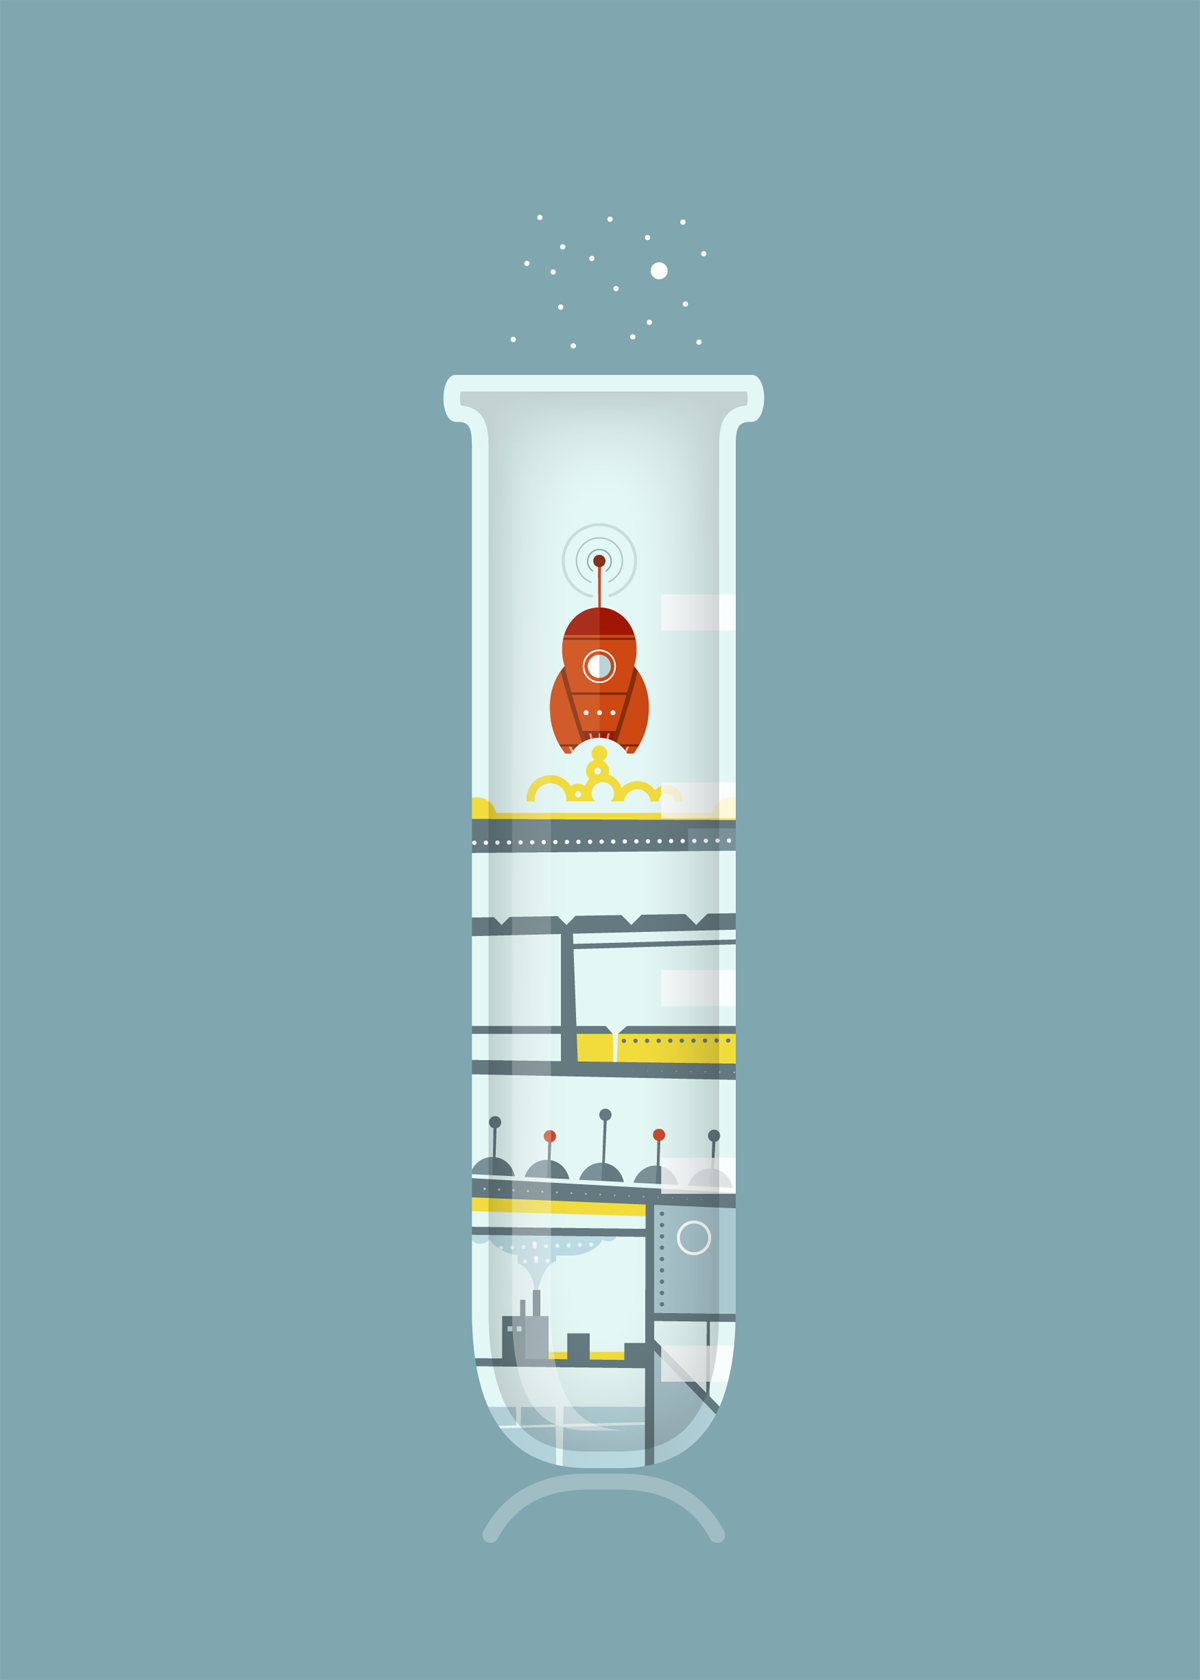
\includegraphics[width=0.51\textwidth]{endmatter/colophon.png}
% \end{figure}

% If you don't want an image in the colophon:
\vspace*{200pt}

\begin{center}
\parbox{200pt}{\lettrine[lines=3,slope=-2pt,nindent=-4pt]{\textcolor{SchoolColor}{T}}{his thesis was typeset} using \LaTeX, originally developed by Leslie Lamport and based on Donald Knuth's \TeX. The body text is set in 11 point Egenolff-Berner Garamond, a revival of Claude Garamont's humanist typeface. The above illustration, ``Science Experiment 02'', was created by Ben Schlitter and released under \href{http://creativecommons.org/licenses/by-nc-nd/3.0/}{\textsc{cc by-nc-nd 3.0}}. A template that can be used to format a PhD thesis with this look and feel has been released under the permissive \textsc{mit} (\textsc{x}11) license, and can be found online at \href{https://github.com/suchow/Dissertate}{github.com/suchow/Dissertate} or from its author, Jordan Suchow, at \href{mailto:suchow@post.harvard.edu}{suchow@post.harvard.edu}.}
\end{center}

\end{document}